In this appendix I show several photos of the ultrapure water system in the same order that the water flows through them.

First of all, the complete scheme of the ultrapure water system is shown in figure \ref{fig:SchemeUPWS}:

\begin{figure}[htbp]
\centering
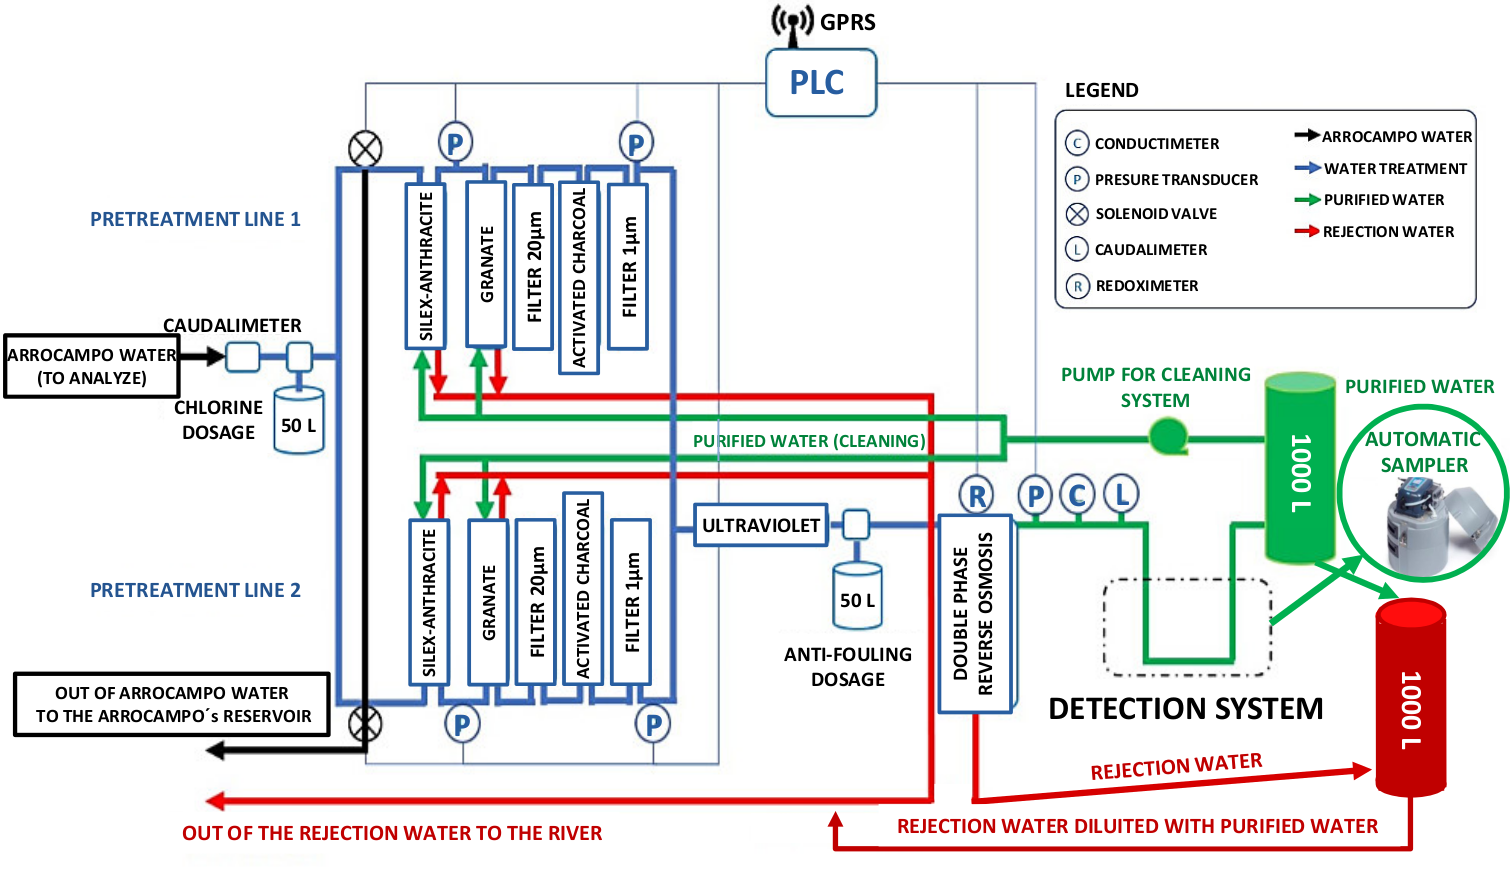
\includegraphics[scale=0.2]{9Appendix/94UltraPureWaterSystem/SchemeUltraPureWaterSystem.png}
\caption{Scheme of the ultrapure water system.\label{fig:SchemeUPWS}}
\end{figure}

Secondly, the Gross filtering stage, made up of Silex-Antracite and Granate filters, is shown in the figure \ref{subfig:GrossFiltering}:

In third place, the fine filtering stage, consisting of $20~\mu\meter$ filter and active carbon filter, is shown in figure \ref{subfig:FineFiltering}:

In fourth place, the superfine filtering, composed of the $1~\mu\meter$ filter and the UV lamps, is shown in the figure \ref{subfig:SuperFineFiltering}

\begin{figure}[htbp]
 \centering
  \subfloat[Gross filtering stage.]{
   \label{subfig:GrossFiltering}
    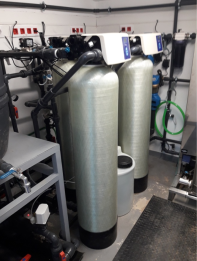
\includegraphics[width=0.3\textwidth]{9Appendix/94UltraPureWaterSystem/GrossFiltering.png}}
  \subfloat[Fine filtering stage.]{
   \label{subfig:FineFiltering}
    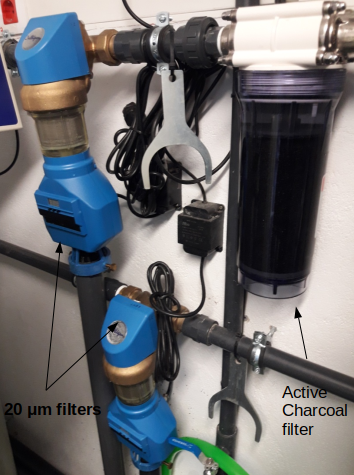
\includegraphics[width=0.3\textwidth]{9Appendix/94UltraPureWaterSystem/FineFiltering.png}}
   %\newline
  \subfloat[Super fine filtering stage.]{
   \label{subfig:SuperFineFiltering}
    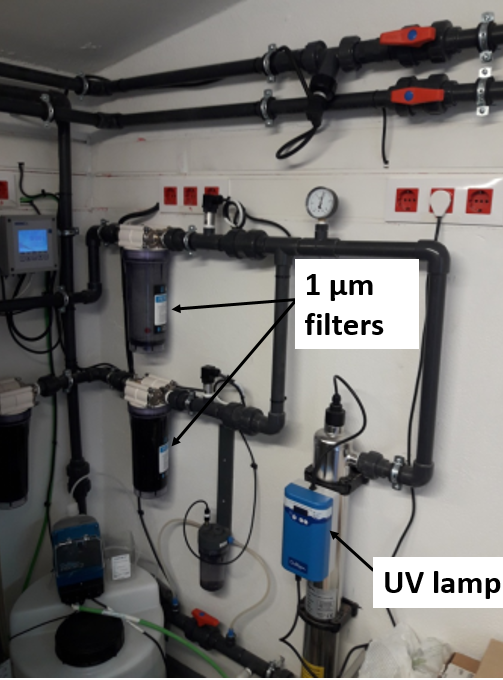
\includegraphics[width=0.3\textwidth]{9Appendix/94UltraPureWaterSystem/SuperFineFiltering.png}}
 \caption{Different stages of filtration of the ultrapure water system.}
 \label{fig:UltraPureWaterStages}
\end{figure}

In fifth place, the double phase reverse osmosis is shown in figure \ref{subfig:Osmosi}

In sixth place, the containers in which we store the ultrapure water and the reject water after treatment is shown in figure \ref{subfig:Containers}.

\begin{figure}[htbp]
 \centering
  \subfloat[Doble phase reverse osmosis stage.]{
   \label{subfig:Osmosi}
    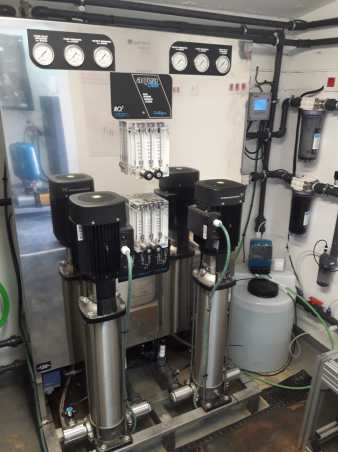
\includegraphics[width=0.3\textwidth]{9Appendix/94UltraPureWaterSystem/Osmosi.png}}
  \subfloat[Storage containers of reject and ultrapure water.]{
   \label{subfig:Containers}
    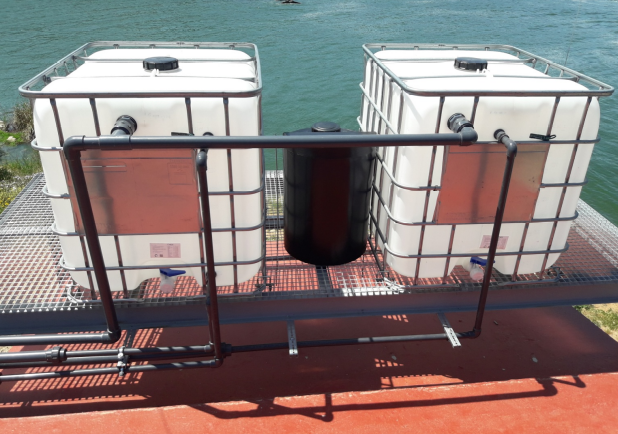
\includegraphics[width=0.5\textwidth]{9Appendix/94UltraPureWaterSystem/Containers.png}}
 \caption{Doble phase reverse osmosis stage and containers used to store the outlet water of the ultrapure water system.}
 \label{subfig:OsmosisContainers}
\end{figure}

In seventh place, the Siemens PLC, software used to control the ultrapure water system, is shown in figure \ref{fig:Siemens}.

\begin{figure}[htbp]
 \centering
  \subfloat[]{
   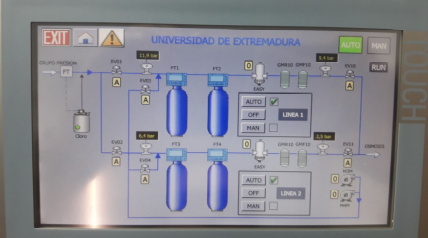
\includegraphics[width=0.37\textwidth]{9Appendix/94UltraPureWaterSystem/Siemens1.png}}
  \subfloat[]{
   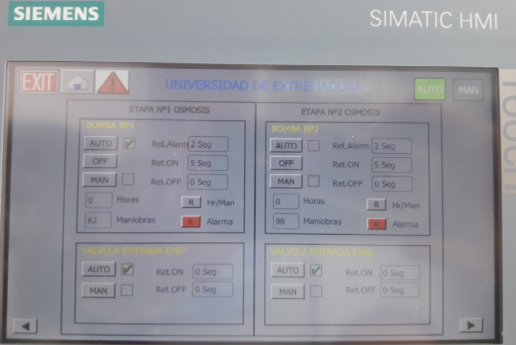
\includegraphics[width=0.3\textwidth]{9Appendix/94UltraPureWaterSystem/Siemens2.png}}
   \subfloat[]{
    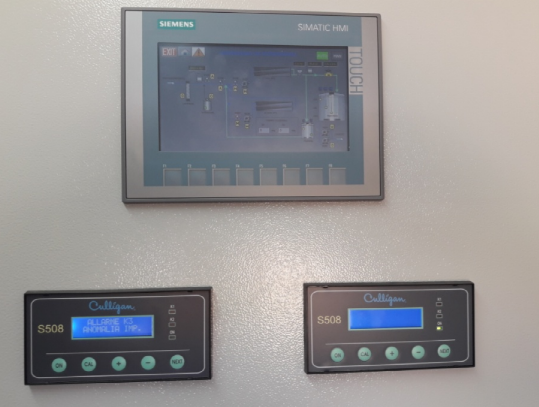
\includegraphics[width=0.27\textwidth]{9Appendix/94UltraPureWaterSystem/Siemens3.png}}
 \caption{Siemens PLC, software for remote control of ultrapure water system.}
 \label{fig:Siemens}
\end{figure}

Finally, the complete system of the ultrapure water system is shown in the figure \ref{fig:CompleteSystem}

\begin{figure}[htbp]
\centering
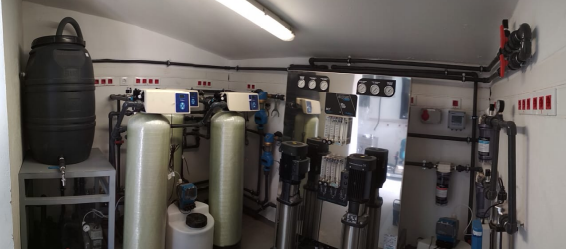
\includegraphics[scale=0.6]{9Appendix/94UltraPureWaterSystem/CompleteSystem.png}
\caption{General photo of the complete ultrapure water system.\label{fig:CompleteSystem}}
\end{figure}

Just as a curiosity, the three types of water (raw water, rejection water and ultrapure water) are shown in figure \ref{fig:ThreeTypesOfWater}, where you can visually check the difference in the tubidity of each type of water.

\begin{figure}[htbp]
\centering
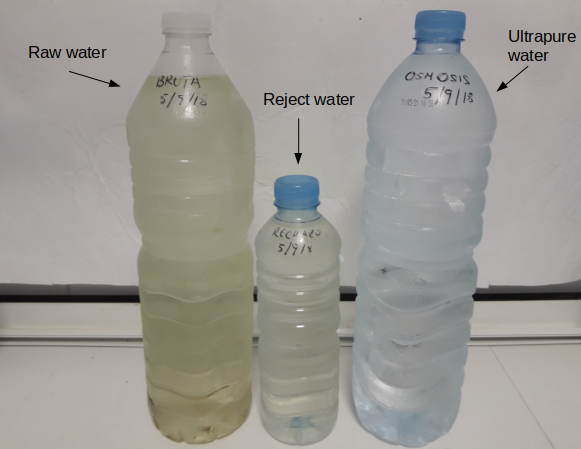
\includegraphics[scale=0.4]{9Appendix/94UltraPureWaterSystem/ThreeTypesOfWater.png}
\caption{Raw water, reject water and ultrapure water obtained with this system.\label{fig:ThreeTypesOfWater}}
\end{figure}
